\hypertarget{group__key__basic}{\section{Basic Methods}
\label{group__key__basic}\index{Basic Methods@{Basic Methods}}
}


Key construction and initialization methods.  


Collaboration diagram for Basic Methods\-:
\nopagebreak
\begin{figure}[H]
\begin{center}
\leavevmode
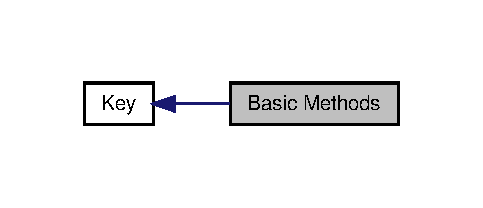
\includegraphics[width=232pt]{group__key__basic}
\end{center}
\end{figure}
Key construction and initialization methods. To use them\-: 
\begin{DoxyCode}
\textcolor{preprocessor}{#include <kdb.h>}
\end{DoxyCode}


Key properties are\-:
\begin{DoxyItemize}
\item \hyperlink{group__keyname}{Key name }
\item \hyperlink{group__keyvalue}{Key value }
\item \hyperlink{group__keymeta}{Key meta data }, including but not limited to\-:
\begin{DoxyItemize}
\item \hyperlink{group__keyvalue_gafb89735689929ff717cc9f2d0d0b46a2}{Key comment }
\item \hyperlink{group__keyname_ga35922a017bee8b4bcb493bbdfad9d6f5}{Key owner }
\item \hyperlink{group__keymeta}{U\-I\-D, G\-I\-D and filesystem-\/like mode permissions }
\item \hyperlink{group__keymeta}{Mode, change and modification times }
\end{DoxyItemize}
\end{DoxyItemize}

Described here the methods to allocate and free the key. 